\section{Background}
\label{sec:background}

Onion services are TCP services that are only accessible over the Tor network.
While conventional Internet services are contacted via their IP addresses, onion
services are contacted via their onion domains, which are resolved and routed
inside the Tor network.  Due to onion services' being hosted in the Tor network,
network traffic traverses six Tor relays (see Figure~\ref{fig:onion-service})
before it reaches the onion service.  The resulting increase in latency is the
cost of the anonymity that onion services provide.

\begin{figure}[t]
\centering
\begin{tikzpicture}[node distance=0.4cm]

\tikzset{>=latex}
\tikzstyle{block} = [rectangle, draw, rounded corners, text centered,
                     minimum height=0.5cm]

\node[block,fill=black!60,
      text=white]         (TB)  {Tor Browser};
\node[block,right=of TB]  (GR1) {Guard};
\node[block,right=of GR1] (MR1) {Middle};
\node[block,below=of MR1] (R)   {Rendezvous};
\node[block,below=of R]   (MR2) {Middle};
\node[block,left=of  MR2] (MR3) {Middle};
\node[block,left=of  MR3] (GR2) {Guard};
\node[block,fill=black!60,
            text=white,
            left=of GR2]  (OS)  {Onion service};

\draw[<->] (TB.east)   -- (GR1.west);
\draw[<->] (GR1.east)  -- (MR1.west);
\draw[<->] (MR1.south) -- (R.north);
\draw[<->] (R.south)   -- (MR2.north);
\draw[<->] (MR2.west)  -- (MR3.east);
\draw[<->] (MR3.west)  -- (GR2.east);
\draw[<->] (GR2.west)  -- (OS.east);

\draw[|-|,gray] ([yshift=3pt] GR1.north west)
                -- node [above, midway, text=gray] {Circuit}
                ([yshift=3pt] MR1.north east);

\draw[|-|,gray] ([yshift=-3pt] GR2.south west)
                -- node [below, midway, text=gray] {Circuit}
                ([yshift=-3pt] MR2.south east);

\end{tikzpicture}
\caption{A connection to an onion service typically consists of six Tor relays.
Both the client and the onion service create a circuit (consisting of two and
three relays, respectively) to the rendezvous relay that serves as a short-lived
data exchange point.}
\label{fig:onion-service}
\end{figure}

As of October 2017, there are approximately 50,000 unique onion services online
each day, as illustrated in Figure~\ref{fig:os-growth}.  The number of Tor users
accessing these onion services is not known because The Tor Project does not
collect such statistics.

\begin{figure}[t]
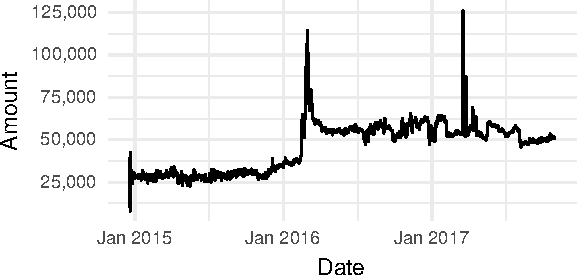
\includegraphics[width=\linewidth]{figures/os-growth.pdf}
\caption{The estimated median number of unique onion services per day since
2015.}
\label{fig:os-growth}
\end{figure}

To create an onion domain, a Tor client first generates an RSA key pair.  It
then computes the SHA-1 hash over the RSA public key, truncates it to 80 bits,
and encodes these 80 bits in Base32, resulting in sixteen characters, \eg,
\texttt{expyuzz4wqqyqhjn}.  As of November 2017, The Tor Project is deploying
the next generation of onion services whose domain format will feature 56
characters~\cite[\S~6]{Mathewson2013a}---a Base32 encoding of the onion
service's public key, a checksum, and a version number.  Because the next
generation uses elliptic curve cryptography, it is possible to make the entire
public key (instead of just a hash over the public key) part of the domain.

Due to an onion domain's being a function of the public key, onion domains are
self-authenticating, meaning that as long as a client has the correct domain, it
knows what public key to expect.  The downside is that sixteen random characters
are impractical to remember, let alone 56 characters.  However, onion domains
can be made at least partially meaningful by repeatedly creating RSA keys until
the resulting domain contains a desired string.  These domains are referred to
as \emph{vanity onion domains}.  A vanity prefix of length $n$ takes on average
$0.5 \cdot 32^n$ key creations given Base32's alphabet size of 32 characters.
After having created a set of domains with a vanity prefix, one can search this
set for the domain that is the easiest to remember, \eg, by using a Markov model
to filter domains that resemble words in the English language.  While this
process will not yield coherent domains, it will greatly facilitate
memorization.

In practice, onion service operators use tools such as scallion~\cite{scallion},
which speed up the process by parallelizing the search for suitable keys.
Vanity domains are used by several organizations such as Facebook
(\url{facebookcorewwwi.onion}), ProPublica (\url{propub3r6espa33w.onion}), and
the New York Times (\url{nytimes3xbfgragh.onion}).

Onion services are private by default.  Once an onion service is created, it is
up to its operator to announce it to the public, \eg, by adding it to onion site
search engines such as Ahmia.\footnote{The search engine is available online at
\url{https://ahmia.fi}.}  The lack of a go-to service such as Google for onion
service discovery prompted the community to devise various ways to publish onion
services; most importantly an array of search engines and curated lists.
